\section{Introduction}
\label{S:intro}
With a technological revolution in mobility on the way, unprecedented changes in urban areas are expected to happen. Before switching to Automated Vehicles (AVs), a careful and detailed investigation is required to analyze their impacts on future mobility patterns, travel behaviour and street design. As a part of human behaviour that is expected to change, interactions between different road users are of importance as they affect safety, efficiency, congestion, quality of service and public trust in transportation systems. In particular, the interaction that we seek to investigate in this study is that of pedestrians, as the most vulnerable road users, and vehicles. Recent instances of AV-pedestrian collisions, e.g. Uber's test AV fatal incident in Tempe, Arizona, and Navya SAS automated bus accident in Vienna, Austria, reveal the vital importance of such investigations. In an urban space dominated by rule-obeying automated vehicles that always stop for pedestrians even at mid-block unsignalized crosswalks, an emphasis on investigating this type of crossing is much needed~\cite{millard2018pedestrians}.
Several questions arise during this investigation: What factors, in terms of traffic parameters, rules and regulations, policies, design, and practices need to be taken into account before the transition toward automated urban environments? Would pedestrians behave differently confronting the yet fairly unknown phenomenon of automated vehicles? And how can we smooth this transition? Moreover, behaviour of pedestrians depend on various factors, e.g. their sociodemographic information, traffic parameters, environmental and lighting conditions, etc~\cite{rasouli2019autonomous}. How can we identify them and their contributions to pedestrian behaviour?

\cref{fig:interaction} depicts a simplified schematic framework of behaviours of different agents involved in a mid-bloc unsignalized cross of a pedestrian. A pedestrian's behaviour in this context can be roughly abstracted into two parts: a) waiting on a sidewalk, during which a pedestrian intends to cross or decides to wait further until they feel more comfortable to cross, and b) crossing the street, which results in a pedestrian trajectory. The driver/vehicle reacts according to its observation of the environment and prediction of pedestrian's behaviour. In this study, we unfold the first part by analyzing pedestrians' waiting time and investigating factors affecting it under different conditions. By focusing on safe crosses of pedestrians, we try to understand what parameters, in term of pedestrians' sociodemographic information, rules and regulations, traffic measures, environmental and vision conditions, etc., affect the time it takes for the pedestrian to start crossing the street. We then propose and discuss possible practices toward transition to pedestrian-friendly automated environments considering the wait time of pedestrians. Wait time of pedestrians throughout this study is associated with safe crossings of pedestrians, without incurring any incidents or discomfort. Shorter wait time before a safe cross can also be associated with more trust in the vehicles, as opposed to longer wait times implying more hesitations to cross safely~\citep{jayaraman2019pedestrian}. Thus, we expect pedestrians who feel more comfortable and confident in the environment to have shorter waiting times.
\begin{figure}
    \centering
    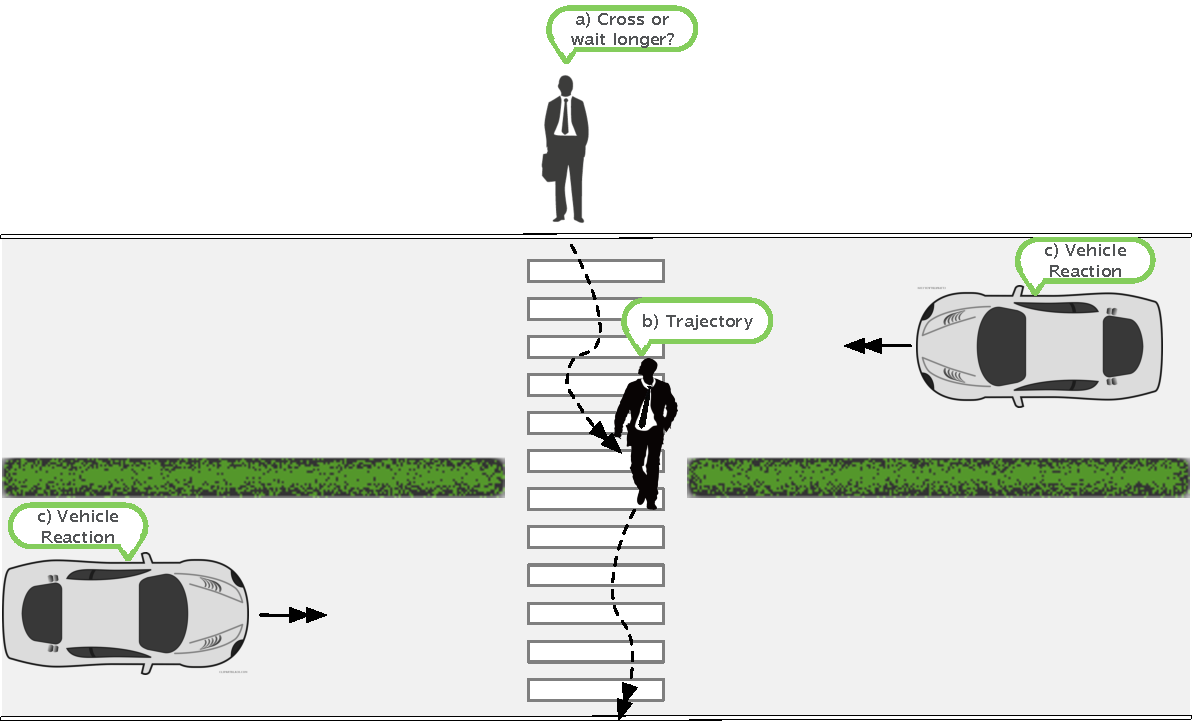
\includegraphics[scale=0.7]{chapter_4/figures/cross.pdf}
    \caption{Schematic representation of vehicles and pedestrians interactions}
    \label{fig:interaction}
\end{figure}

Obtaining data for studies involving pedestrian crossing behaviour is often difficult, as it could be dangerous to participate in various crossing scenarios under different conditions. Related studies mainly rely on data extracted from video footage, which often fail to capture details required for policy suggestions and best practices. Such data are often collected passively from environments with either no or a limited form of control on variables of crossing scenarios. To tackle the difficulties of data collection for studies on futuristic subjects, and to elicit more realistic responses than stated preferences surveys, a virtual reality experiment is designed and implemented in this study, involving around 180 participants over a period of 5 months. 

To analyze the data, a neural network based survival model is developed, and the results are compared to traditional survival models. To enhance the performance of the model and add to its explainability, a feature selection method and a post-hoc game theoretic based interpretability method are added to the framework, respectively. Various researchers have studied the technology, adaption rate, demands, etc. of automated vehicles. However, according to a survey on recognizing the barriers to cities' AV efforts, the lack of clarity on issues that require city actions is pointed out as one of the biggest obstacles for preparing cities for automated vehicles~\citep{kinaSUR}. We try to address such issues by providing detailed insights from our experiments, models, and results.

This paper builds upon our previous work~\citep{kalatian2019deepwait} where an initial deep learning model was proposed for wait time. The current study has been extensively enhanced compared to the earlier work by adding a broader analysis of the data and data collection process, detailed explanations on the virtual reality experiments and their design, more consistent and systematic comparison of the models, a comprehensive analysis of deep learning models' interpretability, and policy and practical recommendations based on the results. We developed suggestions and practical implications which can be useful for urban planners, AV manufacturers, transportation researchers and policy makers. In short, contributions of the current study to the transportation research community can be summarized as follows:
\begin{itemize}
    \item Introducing, developing and utilizing a large-scale virtual reality experiment design and data collection procedure, which is of use for the experiments involving futuristic scenarios as well as situations that might be dangerous for participants to execute in real life.
    \item Developing a data-driven survival model, as well as its detailed and systematic interpretation to analyze the contributing factors to the wait time of pedestrians.
    \item Recommending policy suggestions and practical implications on both virtual reality data collection and pedestrian crossing behaviour. Future studies intending to use virtual reality for data collection can use suggestions to better manage their available resources, and policy makers can use our recommendations as either a validation tool or a ground for deciding on the issues of cities concerning pedestrians and/or automated vehicles.
\end{itemize} 

The rest of this paper is organized as follows: after a brief review of the literature on waiting time studies, pedestrian and automated vehicles interactions, neural network-based survival analysis and machine learning interpretability in \cref{S:lit}, the model is described in detail in \cref{S:meth}, along with the methodology implemented for feature selection and model interpretability. The data collection procedure, from experiment design to data summary is then presented in \cref{S:data}. Model results and analysis are then provided in \cref{S:results}, followed by a discussion of practical implications and policy insights in \cref{S:discuss}. Finally, a conclusion of the research and the future directions of the study will conclude this paper in \cref{S:Con}. 
